

\documentclass[10pt,final,conference,a4paper,twocolumn]{IEEEtran_AntennEMB_GigaHertz2016}
\usepackage{graphicx}



\usepackage[swedish,english]{babel}
\usepackage[bottom]{footmisc}



% The document begins here
\begin{document}

% paper title
\title{Continuous complex permittivity extraction from water-glucose solutions using a resonant microwave cavity around 300 MHz}

% author names and affiliations
\author{Matthias Carlsson$^1$, Gustav Eriksson$^1$, Jens Ljungberg$^1$ and Dragos Dancila$^2$ \\
\em \small \textbf{1:} Student in Master of Eng. Physics, \textbf{2:} Associate Senior Lecturer at Dep. of Eng. Sciences - SSE at Uppsala University \\
\small matthias.carlsson.5845@student.uu.se, gustav.eriksson.0648@student.uu.se, \\
\small jens.ljungberg.2853@student.uu.se and dragos.dancila@angstrom.uu.se
}

\maketitle
\section{INTRODUCTION}
 Complex permittivity is a measure of a dielectric's response to an electric field. Today it is widely used to discern internal changes in a material and/or discern two materials from each other. One particular field which has been recently studied is to monitor the permittivity change of blood at different glucose levels \cite{c2}. Additionally, the authors see industrial applications in monitoring the wear of lube oils or alcohol levels continuously in breweries or wineries.
 
 In this paper a method based on small cavity perturbation theory \cite{c3} is proposed to measure complex permittivity non-evasively and continuously. In the proposed setup the liquid is circulating through a strong electric field (along the z-axis in Fig \ref{fig:sim}). The frequency response around the cavity's resonance frequency is measured by a Virtual Network Analyzer (VNA). The method of determining the permittivty from the frequency response can be found in previous papers \cite{c2}\cite{c1} but with different setups, higher frequencies and higher water-glucose concentrations compared to what are presented in these papers.
 
 The setup is powerful enough to discern a trend in glucose concentrations ranging from 50-200mg/dl, the typical glucose range of human blood. The method is generic and can be used in a variety of situations to monitor small permittivity changes continuously.

\begin{figure}[b]
 	\centering
 	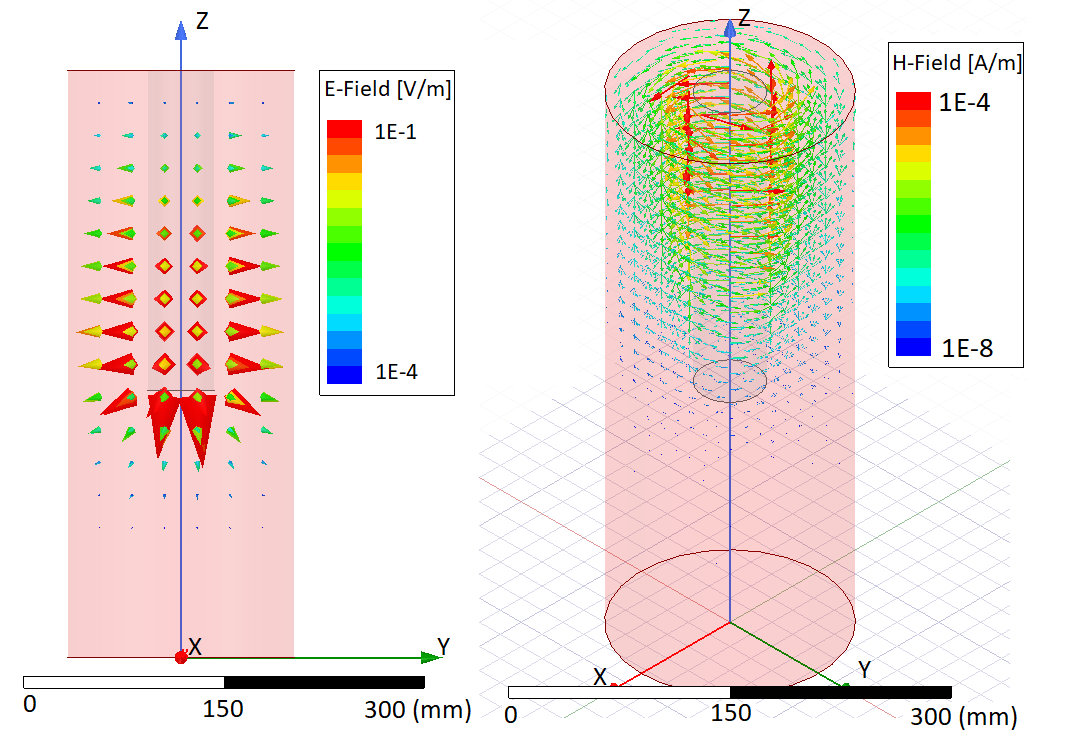
\includegraphics[width=1.0\columnwidth]{EHfield.png}
 	\caption{A simulation of the cavity done in HFFS}
 	\label{fig:sim}
 \end{figure}
\section{EVALUTING THE SETUP/RESULTS}
% \begin{figure}[b]
%	\centering
%	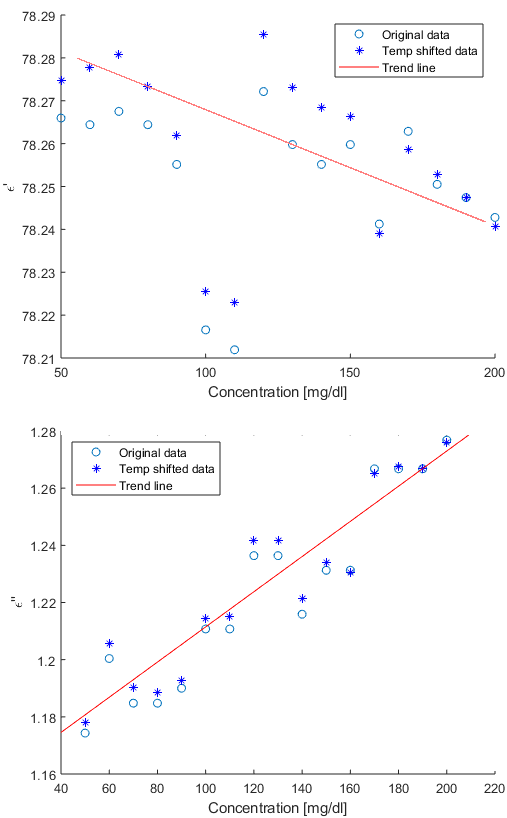
\includegraphics[width=1.0\columnwidth]{pumpgluzoomERE.png}
%	\caption{Re. part of c. permittivity, $\epsilon'$ vs concentration. Shifts in $\epsilon''$ due to small temperature variations. The circles are the original data (No temperature compensation) and the stars are the temperature shifted points}
%	\label{fig:ere}
%\end{figure}
To evaluate the setup, measurements were made of water-glucose solutions with different glucose concentrations. 168(05) $\mu$l of glucose solution with a concentration of 1g/10ml was mixed with 5.00(50) dl DI-water. Between each measurement the concentration was increased by 10 mg/dl. The results are shown in Fig. \ref{fig:eim} where the original measurements are shown as circles and a calculated temperature shift corresponding to a temperature difference between 0 to $\pm$0.007$^o$C are shown as stars.

%\begin{figure}[t]
%	\centering
%	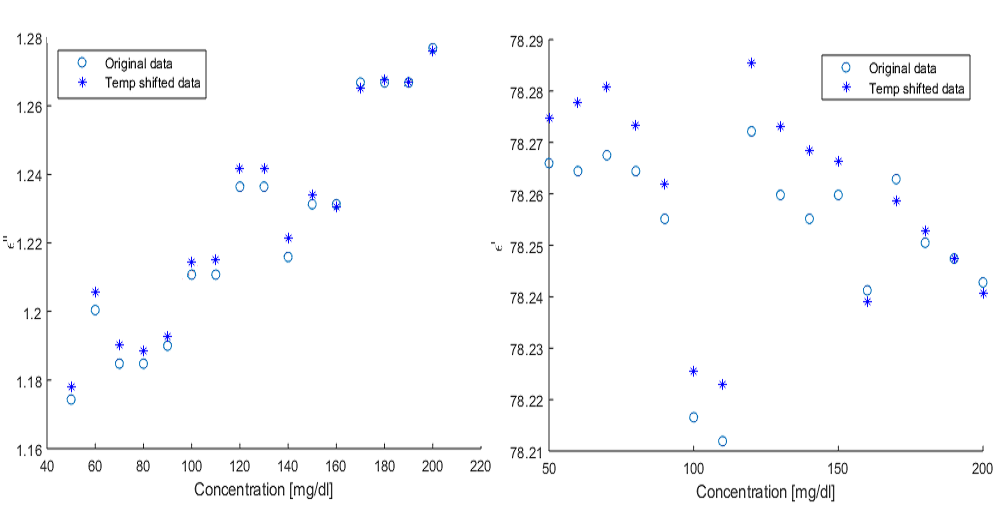
\includegraphics[width=1.0\columnwidth]{pumpgluzoomEIM.png}
%	\caption{Re. part of c. permittivity, $\epsilon''$ vs concentration. Shifts in $\epsilon''$ due to small temperature variations. The circles are the original data (No temperature compensation) and the stars are the temperature shifted points}
%	\label{fig:eim}
%\end{figure}
\begin{figure}
\begin{subfigures}
	\raggedright
	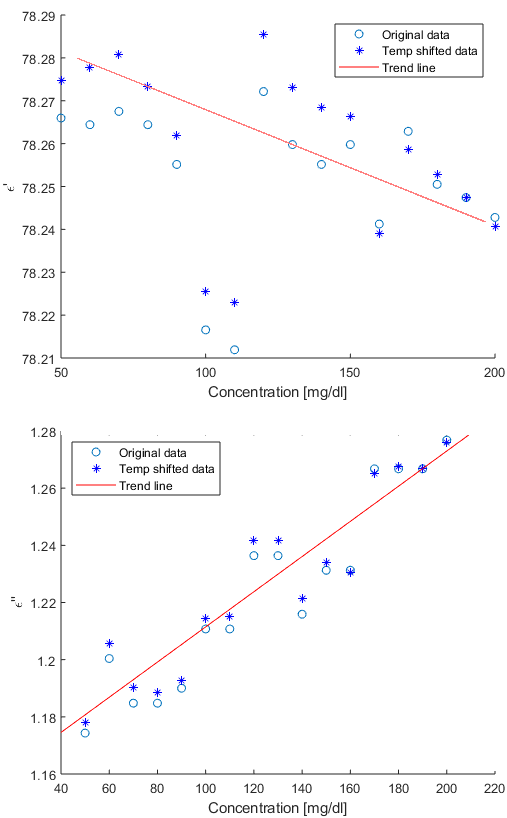
\includegraphics[width=.50\linewidth]{pumpgluzoomERE.png}
	\caption{A subfigure}
	\label{fig:sub1}
\end{subfigures}
\begin{subfigures}
	\raggedright
	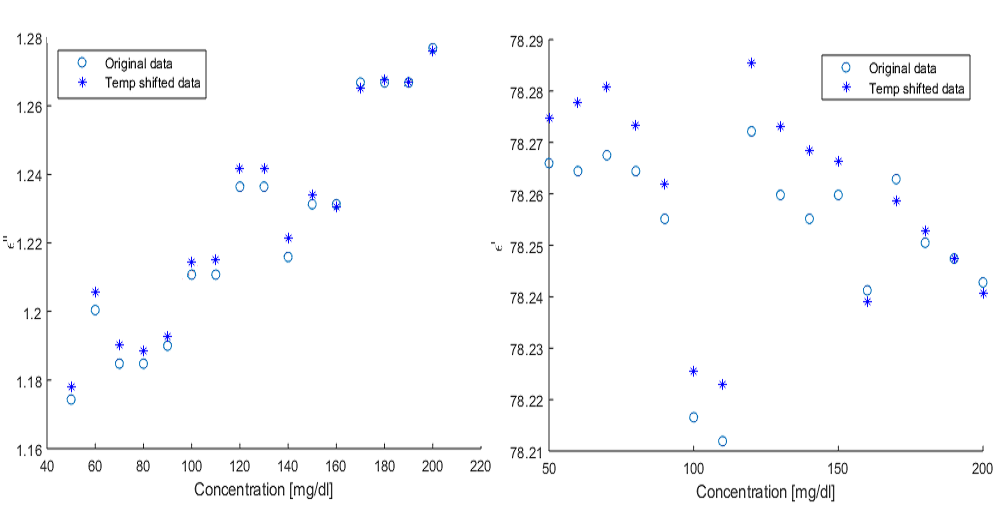
\includegraphics[width=.50\linewidth]{pumpgluzoomEIM.png}
	\caption{A subfigure}
	\label{fig:sub2}
\end{subfigures}
\end{figure}



%\section{CITING PREVIOUS WORK} 
%When referencing a journal article~\cite{hansen84}, a conference digest
%article~\cite{richter01} or a book~\cite{stutzman98} use the usual \LaTeX\ biblio\-graphy environments.



\section{CONCLUSIONS}
In this paper we suggest and evaluate a method of measuring the permittivity in a narrow frequency range around a cavity's resonant frequency. The approach is generic and can be applied to almost any cavity as the procedure only involves redirecting some of the flow to go through the cavity.

In the evaluation we show that the method is accurate enough to result in a trend in a relatively narrow glucose-water concentration range. For improvements, the uncertainty in the permittivity can be reduced by better reference values, more accurate calculations, better concentration and temperature control and a more rigid setup. Despite the many possible improvements we believe that the method as it is, can successfully be used to detect anomalies and deviations in complex permittivity from a reference value.
%\addtolength{\textheight}{-18cm}   % This command serves to balance the column lengths
% on the last page of the document manually. It shortens
% the textheight of the last page by a suitable amount.
% This command does not take effect until the next page
% so it should come on the page before the last. Make
% sure that you do not shorten the textheight too much.




%\section*{ACKNOWLEDGEMENT}  
%The authors wish to acknowledge the assistance and support of all those who
%contribute to...

% references section

% NOTE: BibTeX documentation can be easily obtained at:
% http://www.ctan.org/tex-archive/biblio/bibtex/contrib/doc/

% You can use a bibliography generated by BibTeX as a .bbl file:
%\bibliographystyle{IEEEtran}
%\bibliography{IEEEabrv,mybib}

% <OR>

% manually copy the resulting .bbl file into this document
% and set the second argument of \begin to the number of references
% (used to reserve space for the reference number labels box)
\begin{thebibliography}{99}
	
	
	
	\bibitem{c2} Hofmann, Maximilian and Fischer, Georg and Weigel, Robert and Kissinger, Dietmar, "Microwave-Based Noninvasive Concentration Measurements for Biomedical Applications", in 2013, IEEE T. on M. T. and T., Volume 61, number 5, pages 2195-2204
	
	\bibitem{c3} D. M. Pozar, Microwave Engineering, Chapter 6: Microwave Resonators. John Wiley \& Sons,
	Inc, 2012.
	
	\bibitem{c1} V. Turgul and I. Kale, "Characterization of the complex permittivity of glucose/water solutions for noninvasive RF/Microwave blood glucose sensing," in 2016, . DOI: 10.1109/I2MTC.2016.7520546.
\end{thebibliography}

% A crude (but effective) way to achieve equally high columns (which looks nicer) on the last page is to shorten the page length of the first % column of the
% last page via \enlargethispage{-X.Xcm} where X.X is the value you find that makes the columns equal.
% This hack will have to be adjusted if the document is altered meaning you will have to tweak the value of X.X iteratively and might
% also change the actual positioning of this command within your text.
% The only way to get around this problem is writing a routine inside the class file which actually calculates the print space on the last
% page and adjusts iteratively (but automatically!) the text height on this page.

%\enlargethispage{-18.5cm} %this shortens the last page so that both columns have the same height (use this after you completely finished your paper)
\end{document}
